\section{Deployment View}

Spring Boot is a software framework first and foremost, and it therefore requires a mechanism to be deployed as an artifact for consumption. In this particular case, Spring Boot relies on Maven Central as it's main distribution artifact repository. Users are able to pull down the Spring Boot artifact from Maven Central to use the provided interfaces and functionalities that it offers for Java web application development.

The mechanism by which Spring Boot is deployed is done through their automated server called \texttt{Concourse}. However, the means to get it running in Concourse is not automated. According to the Spring Boot documentation for their continuous integration pipeline, a specific command is issued through the command line to trigger the pipeline. The following is the command to do the aforementioned:\\

\begin{lstlisting}[language=bash, caption={Start Continuous Integration Pipeline Command \cite{springbootconcourse:online}}]
$ fly -t spring-boot set-pipeline -p spring-boot-2.3.x -c ci/pipeline.yml -l ci/parameters.yml
\end{lstlisting}\ \\

In the above command, the file \texttt{ci/pipeline.yml} is a set of instructions to be run from top to bottom. The \texttt{ci/parameters.yml} provides the \texttt{ci/pipeline.yml} file a set of arguments to be passed in through interpolation. On a high level, the pipeline.yml file calls other \texttt{*.yml} files which have their own instructions. These files can be found in the \texttt{ci/tasks} directory and include the following \cite{springboottasks:online}:

\begin{itemize}
\item \textbf{build-deployment-tests.yml}: File that calls the \texttt{ci/scripts/build-deployment-tests.sh} script which initially calls another script called \texttt{common.sh}. The \texttt{common.sh} script will create a soft link between the current working directory's \texttt{embedmongo} file to the home directory and then cleans the local repository of old dependencies. This process will go back to the \texttt{build-deployment-tests.sh} script and run the deployment tests with the embedded \texttt{MongoDB} managed process against a local \texttt{distribution-repository} file.
\item \textbf{build-integration-tests.yml}: File that calls the \texttt{ci/scripts/build-integration-tests.sh} script which initially calls another script called \texttt{common.sh}. The \texttt{common.sh} script will create a softlink between the current working directory's \texttt{embedmongo} file to the home directory and then cleans the local repository of old dependencies. This process will go back to the \texttt{build-integration-tests.sh} script and run the integration tests with the embedded \texttt{MongoDB} managed process against a local \texttt{distribution-repository} file.
\item \textbf{build-project.yml}: File that calls the \texttt{ci/scripts/build-project.sh} script. The script checks the results of the integration tests that were ran to verify that the results meet a specified acceptance criteria, and if it does, then it will proceed to deploy the Spring Boot framework release to the Artifactory repository.
\item \textbf{build-smoke-tests.yml}: File that calls the \texttt{ci/scripts/build-smoke-tests.sh} script which initially calls another script called \texttt{common.sh}. The \texttt{common.sh} script will create a softlink between the current working directory's \texttt{embedmongo} file to the home directory and then cleans the local repository of old dependencies. This process will go back to the \texttt{build-smoke-tests.sh} script and run the smoke tests with the embedded \texttt{MongoDB} managed process against a local \texttt{distribution-repository} file.
\item \textbf{detect-jdk-updates.yml}: File that calls the \texttt{ci/scripts/detect-jdk-updates.sh} script. The script checks that each of their self-managed Docker images of OpenJDK 8, 11, and 13 are up to date with the latest releases. This is done by making a network GET request to\\ \texttt{https://api.adoptopenjdk.net/v2/info/releases/openjdk8} and extracting information from the response. Based on this extraction, the script can determine If there is a need to upgrade any of the aforementioned OpenJDK versions. If there is, then the script will dynamically create an issue on the Spring Boot GitHub repository through a network POST request with the extracted information from the response.
\item \textbf{generate-release-notes.yml}: File that calls the \texttt{ci/scripts/generate-release-notes.sh} script. The script will invoke jar file called \texttt{github-release-notes-generator.jar} with provided arguments that contain GitHub credentials as well as path to the Spring Boot GitHub repository. The end result is a produced file called \texttt{release-notes.md} that is directly put into GitHub. It will also version and tag the release.
\item \textbf{promote.yml}: File that calls the \texttt{ci/scripts/promote.sh} script. The script will define an environment variable called \texttt{BUILD\_INFO\_LOCATION}. The environment variable's value gives a path to a json file called \texttt{build-info.json} on the local machine, which in itself contains information about their Artifactory repository. Using the environment variable, the \texttt{promote.sh} script promotes and distributes through the various stages which has an associated release type, namely: milestone, release candidate, and release. After this, the script publishes the Spring Boot artifact as a plugin.
\item \textbf{stage.yml}: File that calls the \texttt{ci/scripts/stage.sh} script. The script will locally pull down a copy of the Spring Boot project from GitHub and deploy it to a Artifactory repository based on the release type. Then, it will run all smoke, integration, and deployment tests against that deployed artifact.
\item \textbf{sync-to-maven-central.yml}: File that calls the \texttt{ci/scripts/sync-to-maven-central.sh} script. The script will synchronize the release artifact in Artifactory repository to the Maven Central repository.
\end{itemize}

Each of the files have their own purpose and concern, and are called at different times of the pipeline but it is important to remember that it is ultimately the \texttt{pipeline.yml} that orchestrates all of the above functionalities of the automated pipeline. Figure ~\ref{deployment-diagram} shows the relationship between the runtime components during the automated pipeline process:

\begin{figure}[H]
    \centering
    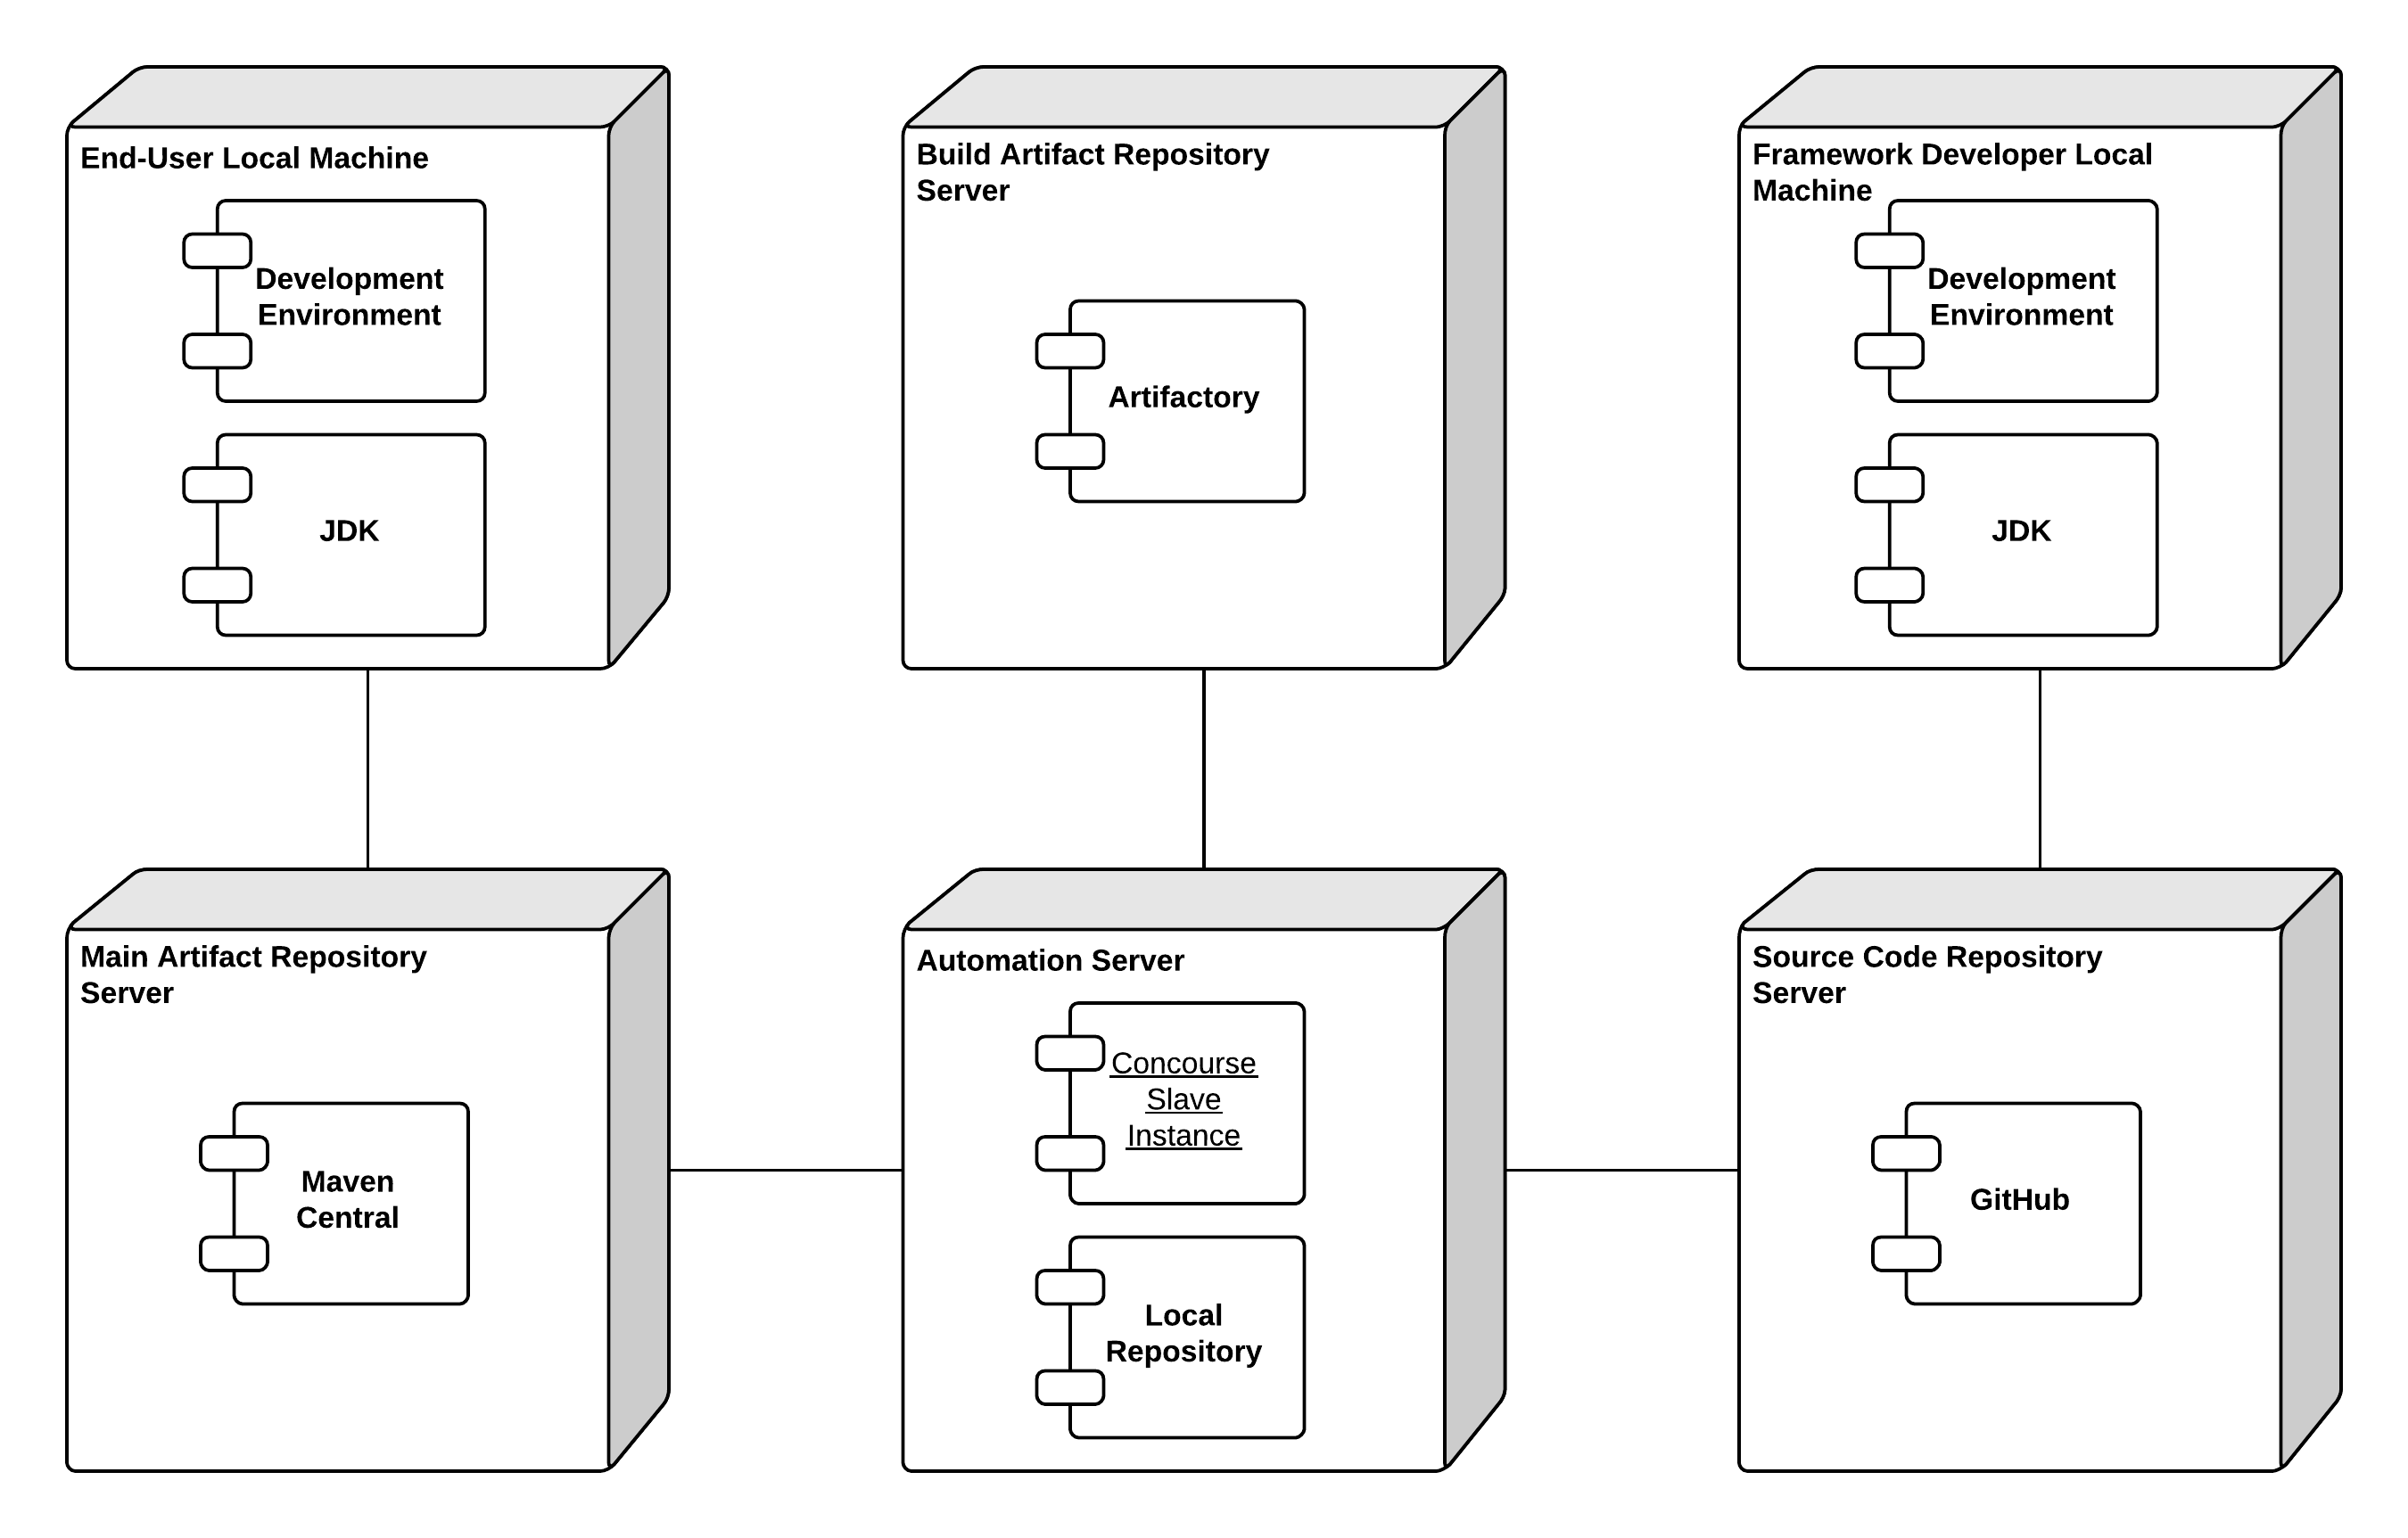
\includegraphics[width=\textwidth]{content/architectural-views-top-level/deployment-diagram.png}
    \caption{Spring Boot Deployment Diagram}
    \label{deployment-diagram}
\end{figure}

The goal of this automated pipeline process is to give releases of the Spring Boot framework to end-users. End-users in this context, being Java developers who want to create web applications quickly. They can integrate the Spring Boot framework into their projects by sourcing it from the Maven Central repository and declaring it as a dependency in their dependency management tool. The following dependency definition below shows generically how it can be sourced and declared:\\

\clearpage

\begin{lstlisting}[caption=Representation of Dependency Management for Spring Boot]

plugins {
	id 'java'
    id 'org.springframework.boot' version '2.2.1.RELEASE'
	id 'io.spring.dependency-management'
}

repositories {
    mavenCentral()
}

dependencies {
    implementation 'org.springframework.boot:spring-boot-starter-web'
    implementation 'org.springframework.boot:spring-boot-starter-data-mongodb'
}
\end{lstlisting}\ \\

This is the final step to get the Spring Boot framework in the hands of Java developers to build their web application.